\documentclass[tikz,border=2mm]{standalone}

\begin{document}
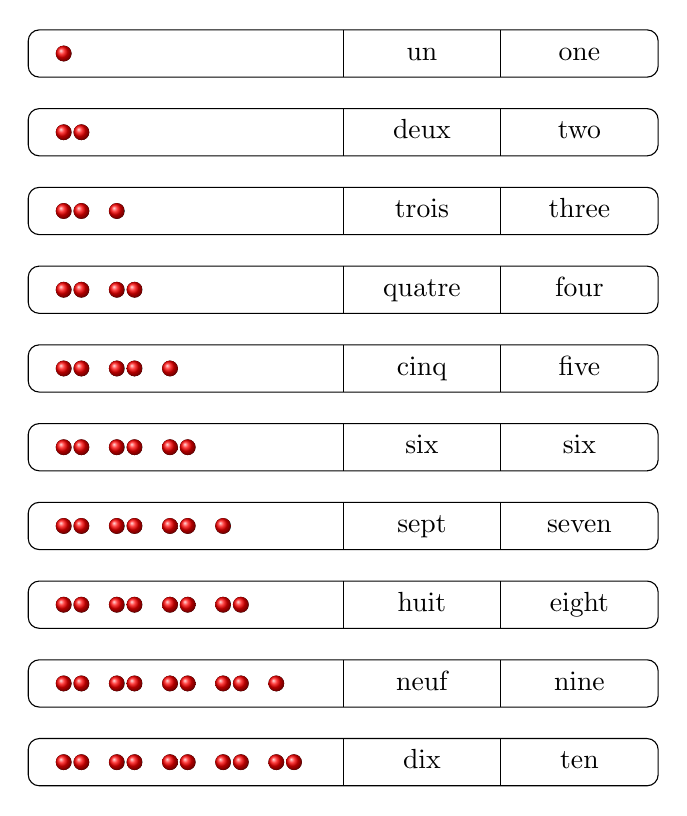
\begin{tikzpicture}
\foreach[count=\ii]\i/\j in
{
  un/one,
  deux/two,
  trois/three,
  quatre/four,
  cinq/five,
  six/six,
  sept/seven,
  huit/eight,
  neuf/nine,
  dix/ten
}
{
  \begin{scope}[shift={(0,-\ii)}]
    \draw[rounded corners] (0,-0.3) rectangle (8,0.3);
    \foreach\k in {4,6}
      \draw (\k,-0.3) -- (\k,0.3);
    \node at (5,0) {\strut\i};
    \node at (7,0) {\strut\j};
    \foreach\k in {1,...,\ii}
      \fill[shading=ball,ball color=red] ({0.225*\k+0.225*int((\k+1)/2)},0) circle (0.1);
  \end{scope}
}

\end{tikzpicture}
\end{document}